\scanpage{69}\mspage{68}
engendrée par la réunion)
% Figure R3-01: the raised correction and its descending leader, with adjoining words once.
\figure{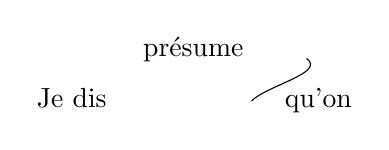
\begin{tikzpicture}[x=1cm,y=1cm]
  \node[anchor=base west] at (0,0) {Je \deleted{dis}};
  \node[anchor=base west] at (1.35,.65) {\inserted{présume}};
  \node[anchor=base west] at (3.15,0) {qu'on};
  \draw (3.55,.62) .. controls (3.8,.44) and (3.05,.28) .. (2.85,.08);
\end{tikzpicture}}
a en fait une algèbre de Boole
% Figure R3-02: opening quotes and ultra are raised; the curved leader is not a hyphen.
\figure{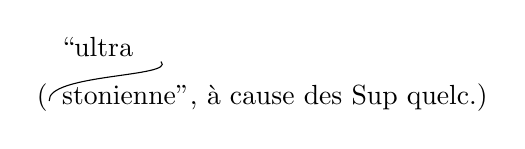
\begin{tikzpicture}[x=1cm,y=1cm]
  \node[anchor=base west] at (0,0) {(};
  \node[anchor=base west] at (.3,.62) {\inserted{``ultra}};
  \node[anchor=base west] at (.32,0) {stonienne'', à cause des $\mathrm{Sup}$ quelc.)};
  \draw (1.7,.55) .. controls (1.9,.35) and (.25,.4) .. (.28,.05);
\end{tikzpicture}}

% slanted
\margin{Cela sera valable dans ``le cas ensembliste'', et en tous cas dans les exemples types, donnés \deleted{\unsure{tout}} au début, en termes d'un $E$ (top. ou mesurable), alors $\Sigma$ s'identifie à l'ens des parties de $E$, et \unsure{on trouvera|on trouve} le compactifié de Stone de $E_{\mathrm{disc.}}$ Dans le cas qui vient, \unsure{je} \unsure{ne vois} comment \unsure{prouver}, pour trois supports
\[
P,Q,R\quad P\wedge(Q\vee R)=\unsure{(|\{}(P\wedge Q)\vee(P\wedge R)\unsure{.|,|)}
\]
}

\deleted{Il faudra y revenir}

Donc les supports \unsure{s'identifient|s'identifieraient} aux \unsure{Parties|Partie} à la fois ouvertes et fermées du spectre, qui serait un espace \deleted{\unsure{to|tot}}\unsure{cpct|cpt|compact} \deleted{\unsure{tot}} \unsure{disconnexe} ultra.stonien.

L'involution correspond au passage au complémentaire.

On fera attention que la construction $\Sigma$ ne dépend que de l'ens ordonné
% Figure R3-03: the long insertion line and the smaller lower insertion enclosure.
\figure{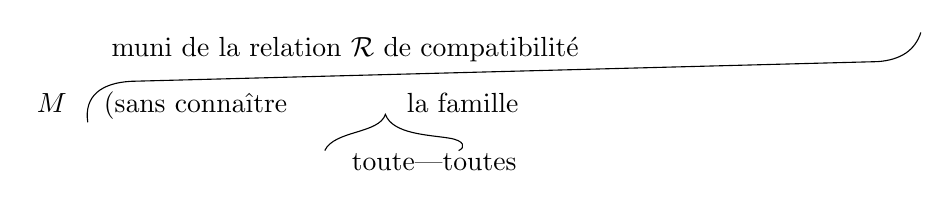
\begin{tikzpicture}[x=1cm,y=1cm]
  \node[anchor=base west] at (0,0) {$M$};
  \node[anchor=base west] at (.85,0) {(sans connaître};
  \node[anchor=base west] at (4.7,0) {la famille};
  \node[anchor=base west] at (.95,.72) {\inserted{muni de la relation $\mathcal R$ de compatibilité}};
  \draw (.77,-.12) .. controls (.72,.22) and (.95,.38) .. (1.32,.4)
    -- (10.8,.65) .. controls (11.1,.67) and (11.28,.8) .. (11.35,1.02);
  \node[anchor=base west] at (4.0,-.73) {\inserted{\unsure{toute|toutes}}};
  \draw (3.78,-.48) .. controls (3.9,-.22) and (4.47,-.27) .. (4.55,-.02)
    .. controls (4.64,-.27) and (5.1,-.28) .. (5.35,-.32)
    .. controls (5.56,-.35) and (5.57,-.44) .. (5.48,-.48);
\end{tikzpicture}}
des parties $\unsure{\overline\Phi|\Phi'|\Phi}$ de $M$, correspondant aux figures). En effet, en termes de $(M,\leq,R)$, le cosupport d'une partie $M'$ de $M$ est défini par
\[
\operatorname{cosup}_M(M')=\{\,x\in M\mid(x,x')\in\mathcal R\quad\forall x'\in M'\,\}
\]

% slanted margin note, transcribed once with its adjoining long rule in Figure R3-04.
\figure{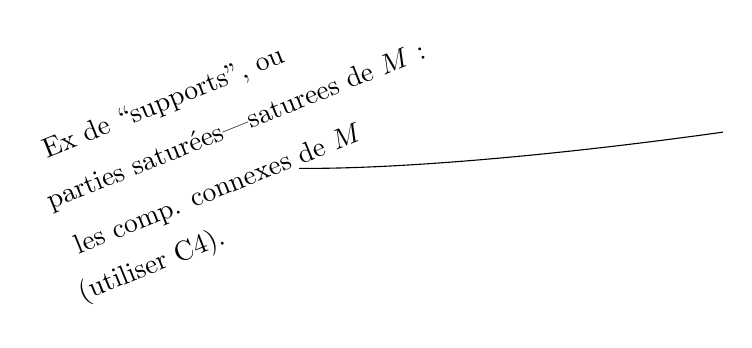
\begin{tikzpicture}[x=1cm,y=1cm]
  \node[anchor=base west,rotate=22] at (0,0) {\uline{Ex} de ``supports'', ou};
  \node[anchor=base west,rotate=22] at (.05,-.65) {parties \unsure{saturées|saturees} de $M$ :};
  \node[anchor=base west,rotate=22] at (.4,-1.22) {les comp. connexes de $M$};
  \node[anchor=base west,rotate=22] at (.45,-1.82) {(utiliser C4).};
  \draw (3.32,-.08) .. controls (4.65,-.09) and (6.7,.1) .. (8.7,.38);
\end{tikzpicture}}
